\subsection{Spielwelt}
Für die Welt, in welcher das Spiel gespielt wird, stehen mehrere Optionen zur Verfügung.

\subsubsection{Gridless}
Die erste Möglichkeit einer Spielwelt ist eine Karte ohne dargestelltes oder vorhandenes Grid. Solch ein System verwendet beispielsweise \textit{Age of Mythology}, wobei die Karte nicht in ein Grid, sondern viele tausende  Koordinaten eingeteilt ist. Diese Form der Positionierung ist daher gängig für \textit{Real Time Strategy} Spiele.

\subsubsection{Square Grid}
Eine weitere Möglichkeit zur Positionierung von Gebäuden oder Einheiten innerhalb einer Spielwelt ist ein \textit{Square Grid} (vgl. \autoref{image:squaregrid}), also die Einteilung der Karte in eine gewisse Anzahl von Quadraten, welche als eigene Felder agieren und worauf Gebäude oder Einheiten zugreifen können. Dieses System wird unter anderem in \textit{Starcraft II} oder \textit{Age of Empires} verwendet, wodurch auch diese Form der Positionierung gängig für \textit{Real Time Strategy} ist. Allerdings findet man diese Eigenschaft auch in \textit{Turn Based Strategy}, darunter die älteren Teile der \textit{Civilization}-Reihe. Dieses System wurde im Laufe der Jahre jedoch von einem Square Grid auf ein Hex Grid umgestellt.

\begin{figure}
    \begin{center}
        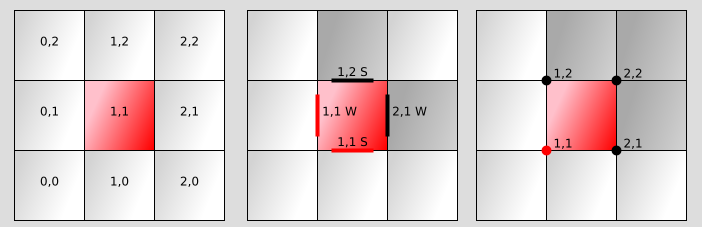
\includegraphics[width=300px]{0.bilder/squaregrid.png}
    \end{center}
    \caption{Aufbau eines Square Grids (\cite{world:grids})} \label{image:squaregrid}
\end{figure}

\subsubsection{Hex Grid}
Die letzte Möglichkeit ist ein \textit{Hex Grid}, welches vor allem Anklang findet im Genre der \textit{Turn Based Strategy} Games, darunter \textit{Endless Legend}, \textit{Civilization VI} und \textit{Humankind}. Der klare Vorteil von einem Grid bestehend aus Hexagonen ist die \textit{Distanzberechnung} und die Anzahl \textit{direkter Nachbarn}. Im Vergleich zu einem Quadrat besitzt ein Hexagon in einem Grid 6 statt 4 direkter Nachbarn, wobei direkt bedeutet, dass die Kanten aneinander angrenzen. Um einen diagonalen Weg in einem Square Grid einzuschlagen, muss ein weiterer Weg aufgewendet werden, da nach dem \textit{Satz des Pythagoras} gilt:
\begin{equation}
    a^2 + b^2 = c^2
\end{equation}
Der diagonale Weg innerhalb eines Quadrates mit Länge 1 und Breite 1 wäre folglich 
\begin{equation}
    \sqrt{1^2 + 1^2} = \sqrt{2}
\end{equation}
Wobei offensichtlich gilt, dass
\begin{equation}
    \sqrt{2} > 1
\end{equation}
Möchte man also Bewegungen von Einheiten in 6 statt 4 Richtungen ermöglichen, empfiehlt sich ein Hex Grid statt einem Square Grid. Die Distanz zwischen allen gegenüberliegenden Kanten eines Hexagons ist stets gleichlang (vgl. \autoref{image:hexgrid}). Unter der Berücksichtigung, dass die Thematik der Bienen auch mit \textit{Bienenwaben} und deren hexagonalen Form assoziiert wird, wird der Prototyp ein Hex Grid verwenden. 
\begin{figure}
    \begin{center}
        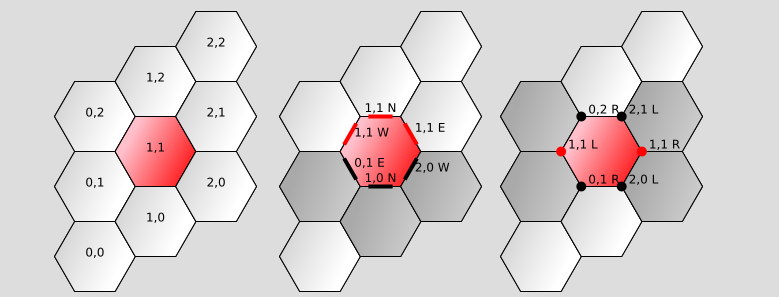
\includegraphics[width=300px]{0.bilder/hexgrid.png}
    \end{center}
    \caption{Aufbau eines Hex Grids (\cite{world:grids})} \label{image:hexgrid}
\end{figure}